\documentclass[a4paper,10.5pt]{ctexart}
\usepackage[left=2.50cm, right=2.50cm, top=2.50cm, bottom=2.50cm]{geometry} %页边距
\usepackage{amsmath}
\usepackage{amssymb}
\usepackage{ctex}
\usepackage{braket}
\usepackage[table,xcdraw]{xcolor}
\usepackage[european]{circuitikz}
\usepackage{multirow}
\usepackage{float}
\usepackage{bm}         % 加粗方程字体
\usepackage{graphicx}
\usepackage{geometry}
\usepackage{helvet}
\usepackage[english]{babel}
\usepackage{booktabs}
\usepackage{indentfirst}
\geometry{left=2.0cm,right=2.0cm,top=2.0cm,bottom=2.0cm}
\usepackage{textcomp}
\usepackage{physics}
%\usepackage{algorithm}
%\usepackage{algorithmic}
\usepackage{longtable}
\usepackage{array}
\usepackage{xcolor}
\usepackage{algpseudocode}
\usepackage{epsfig}
\usepackage{arydshln}
%\usepackage[boxed]{algorithm2e}

\usepackage{algorithm,algpseudocode,float}
\usepackage{lipsum}
\makeatletter
\newenvironment{breakablealgorithm}
  {% \begin{breakablealgorithm}
   \begin{center}
     \refstepcounter{algorithm}% New algorithm
     \hrule height.8pt depth0pt \kern2pt% \@fs@pre for \@fs@ruled
     \renewcommand{\caption}[2][\relax]{% Make a new \caption
       {\raggedright\textbf{\ALG@name~\thealgorithm} ##2\par}%
       \ifx\relax##1\relax % #1 is \relax
         \addcontentsline{loa}{algorithm}{\protect\numberline{\thealgorithm}##2}%
       \else % #1 is not \relax
         \addcontentsline{loa}{algorithm}{\protect\numberline{\thealgorithm}##1}%
       \fi
       \kern2pt\hrule\kern2pt
       \renewcommand{\algorithmicensure}{\textbf{Output:}}
     }
  }{% \end{breakablealgorithm}
     \kern2pt\hrule\relax% \@fs@post for \@fs@ruled
   \end{center}
  }
\makeatother

\usepackage{listings} 
\usepackage{xcolor}

\lstset{
  language=Matlab,  %代码语言使用的是matlab
  frame=shadowbox, %把代码用带有阴影的框圈起来
  rulesepcolor=\color{white!},%代码块边框为淡青色
  keywordstyle=\color{blue!90}\bfseries, %代码关键字的颜色为蓝色,粗体
  commentstyle=\color{white!20!black!60!}\textit,    % 设置代码注释的颜色
  showstringspaces=false,%不显示代码字符串中间的空格标记
  numbers=left, % 显示行号
  numberstyle=\tiny,    % 行号字体
  stringstyle=\ttfamily, % 代码字符串的特殊格式
  breaklines=true, %对过长的代码自动换行
  extendedchars=false,  %解决代码跨页时,章节标题,页眉等汉字不显示的问题
   escapebegin=\begin{CJK*},escapeend=\end{CJK*},      % 代码中出现中文必须加上,否则报错
  texcl=true}



\newcommand{\PreserveBackslash}[1]{\let\temp=\\#1\let\\=\temp}
\newcolumntype{C}[1]{>{\PreserveBackslash\centering}p{#1}}
\newcolumntype{R}[1]{>{\PreserveBackslash\raggedleft}p{#1}}
\newcolumntype{L}[1]{>{\PreserveBackslash\raggedright}p{#1}}
\renewcommand{\algorithmicrequire}{ \textbf{Input:}}       
\renewcommand{\algorithmicensure}{ \textbf{Initialize:}} 
\renewcommand{\algorithmicreturn}{ \textbf{Output:}}     

%算法格式
\usepackage{fancyhdr}
\usepackage{subfigure}
\pagestyle{plain}

\lhead{}
\chead{}
\lfoot{}
\cfoot{}
\rfoot{}
\usepackage{hyperref} %bookmarks
\hypersetup{colorlinks, bookmarks, unicode} %unicode
\usepackage{multicol}



\title{\textbf{基于求解非线性方程组的椭圆面积估计}}
\date{}



\begin{document}

	\maketitle
\begin{center}
\Large{\bf {摘\qquad 要}}
\end{center}


%解决了什么问题、应用了什么方法、得到了什么结果;文字简练,突出新见解、新方法;最后书写(1000)
\par %开头段:充分概括论文内容,两到三句话:简单交代题目背景;交代我们所做的事情(重要);这个问题的实际意义(可省)
在生产流程中,为了迅速计算近似椭圆的平面图形,某公司采用在椭圆平面内设置摄像机并通过分析所摄线段长度计算面积的方法。目前考虑特殊情况,即等距摆放三个对准圆心的摄像机,本文对于问题一、二中椭圆的不同情境,从解析几何的理论出发,基于椭圆和直线方程,建立两种情况下的面积求解模型。该模型可用于计算在上述摆放情形下,给定相应参数,椭圆在圆各个相对位置下的近似面积。
\par \textbf{针对问题一:}%解决了什么问题、应用了什么方法(一定要结合题目说明)、得到了什么结果(计算数值答案/开放题简要答主要部分)
该问题中摄像机的角度、椭圆的长轴、短轴视为未知量。我们认为相对于圆周,椭圆足够小,因此我们首先建立摄像机所作两条平行切线切于椭圆的几何模型,通过建立关于三个已知量$(a,b,c)$与三个未知量$(l,k,\theta)$的方程,无需添加摄像头个数即可测出面积近似值。使用MATLAB软件编程,运用$vpasolve$等函数,求解出半长轴、半短轴等参数,并得到面积近似值$S$,存入表格,并最终通过误差分析得到:随着$l$,$k$,$\theta$的变化,面积误差的数量级均控制在$10^{-13}$以内。同时考虑椭圆退化为圆或者线段的情况,得到结论:当所观测图形为线段时,满足$a=b+c$或$a=b-c$;当所观测图形为圆时,满足$a=b=c$。
\par \textbf{针对问题二:}该问题较问题一更为贴近现实,其中除了摄像机的角度、椭圆的长轴、短轴,圆心的位置也为共同影响变量,相较于问题一而言,不再假设摄像机发出的两条切线平行,需要考虑过摄像机作两条切线。在刻画三条线段与圆心的偏离程度时,若照片中所示圆心在线段上,则观测圆心与两端点的距离之差的绝对值;若照片中所示圆心在线段外,则观测圆心与两端点的距离之和。因此我们再次建立几何模型,围绕椭圆半长轴、半短轴、圆心位置、摄像机夹角和线段与圆心偏离距离,基于椭圆方程、切线方程、弦长方程等解析几何理论知识,建立关于六个已知量$(a,b,c,d_1,d_2,d_3)$和五个未知量$(x_0,y_0,\theta,l,k)$的方程组,无需添加摄像头个数即可测出面积近似值。使用MATLAB软件编程,主要运用$solve$、$vpasolve$等核心函数,求出半长轴、半短轴等参数,并得到面积的近似值$S$。利用几组数据考察代码的求解情况,与真实值进行比较后发现相对误差控制在$0.5\%$内。
\\
\noindent{\bf 关键词:}平面直角坐标系\quad MATLAB\quad 非线性方程组\quad 解析几何
\clearpage

\section{问题重述}
%数学建模比赛论文是要我们解决一道给定的问题,所以正文部分一般应从问题重述开始,一般确定选题后就可以开始写这一部分了。
%这部分的内容是将原问题进行整理,将问题背景和题目分开陈述即可,所以基本没啥难度。
%本部分的目的是要吸引读者读下去,所以文字不可冗长,内容选择不要过于分散、琐碎,措辞要精练。
%注意:在写这部分的内容时,绝对不可照抄原题!(论文会查重)
%应为:在仔细理解了问题的基础上,用自己的语言重新将问题描述一遍。语言需要简明扼要,没有必要像原题一样面面俱到。
\par 为了快速计算近似椭圆的平面图形的面积,可以在椭圆所在平面设置$n$台摄像机拍摄$n$张图片,并根据拍摄得到的$n$条线段长度计算近似面积。当下,在直径约1米的圆周上等距设置3台对准圆心$O$的摄像机,待测量平面物体被置于圆心附近。
\par 下面针对以下两种情况解决问题:
\par \textbf{问题一}:在待测量物体直径远小于圆周直径,不超过$5$cm,且中心位于大圆周圆心的状态下,试利用拍摄得到的线段长,建立数学模型给出椭圆面积的近似公式;进一步,研究椭圆为圆和线段时所满足的条件。
\par \textbf{问题二}: 在待测量物体位于以$O$为圆心,半径为$20$cm的圆中的状态下,试利用拍摄得到的线段段长和线段端点至圆心的偏离距离,建立数学模型给出误差不超$0.5\%$的面积近似公式;若误差不达标,可以增加摄像机个数进行方案调整,并说明原因。
\section{问题分析}
\subsection{问题一的分析}
将此问题在二维平面上进行考虑。欲计算椭圆的面积,需要求出椭圆的半长轴和半短轴长度,同时椭圆长轴与三台摄像机的偏离角度也是未知量。由于三台摄像机是在圆周上等距放置,因此只需设出其中一台摄像机与椭圆长轴的偏离角度。因此,对于此问题,已知量为三条线段的长度,未知量为椭圆的半长轴、半短轴以及某一台摄像机与椭圆长轴的偏离角度,我们尝试建立三个已知量与三个未知量之间的方程,从而解出椭圆的半长轴、半短轴,计算出椭圆面积。
\begin{figure}[h]%h可替换成t表示在页首插入图片;b页尾;p整页
\centering
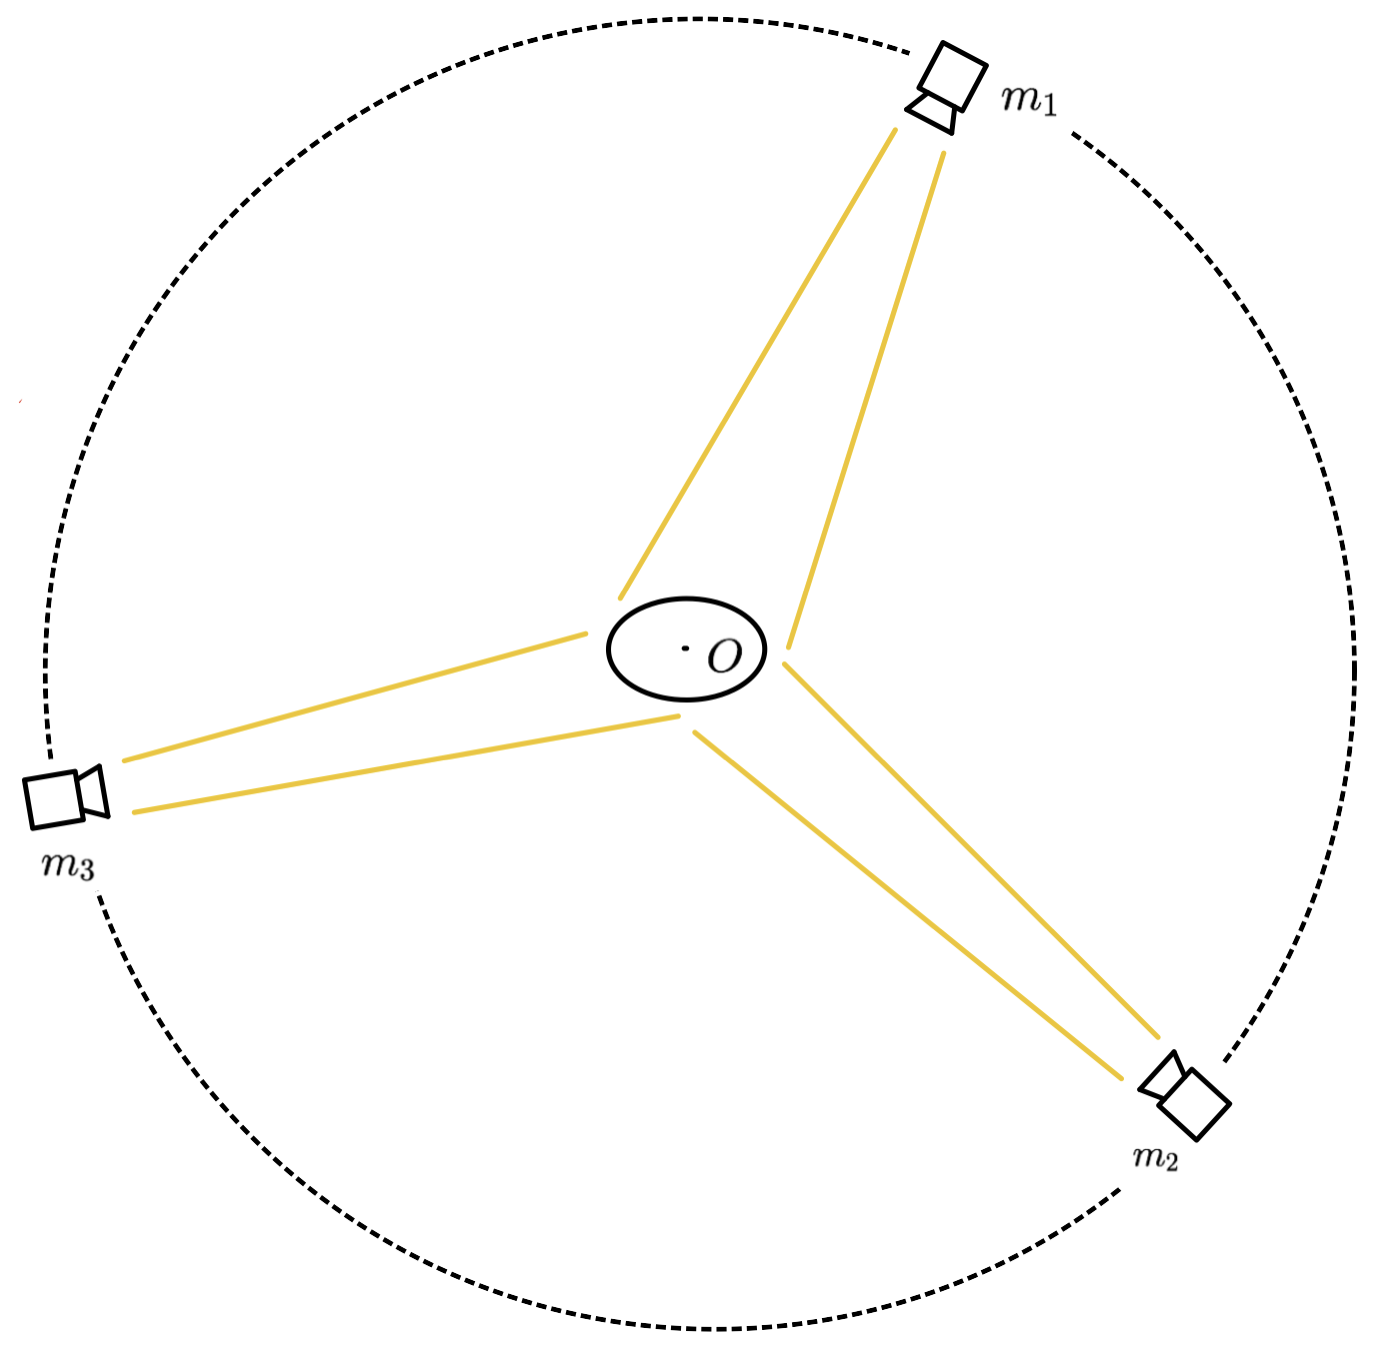
\includegraphics[scale=0.28]{示意图.png}
\caption{问题1示意图}
\label{fig:label}
\end{figure}
\subsection{问题二的分析}
\par 和问题一的背景类似,问题二中平面图形被限制在半径为$20$cm的同心圆中,其中心可能不再与圆心重合,且摄像机所做切线不平行。现以椭圆圆心$O$为原点,长轴正方向为$x$轴建立坐标系。欲计算椭圆的面积,仍需求出椭圆的半长轴和半短轴长度,同时圆心的坐标$(x_0,y_0)$和摄像机与椭圆长轴偏离角度也是未知量。因此,对于此问题,已知量为三条线段长度和三个线段与圆心偏离度,在刻画三条线段与圆心的偏离程度时,若照片中所示圆心在线段上,则观测圆心与两端点的距离之差的绝对值;若照片中所示圆心在线段外,则观测圆心与两端点的距离之和。未知量为椭圆的半长轴、半短轴、圆心的横纵坐标以及某一台摄像机与椭圆长轴的偏离角度。利用几何关系,我们尝试建立五个未知量和六个已知量之间的方程,并借助MATLAB等工具,从而解出椭圆的半长轴、半短轴,计算出椭圆面积。
\begin{figure}[h]%h可替换成t表示在页首插入图片;b页尾;p整页
\centering
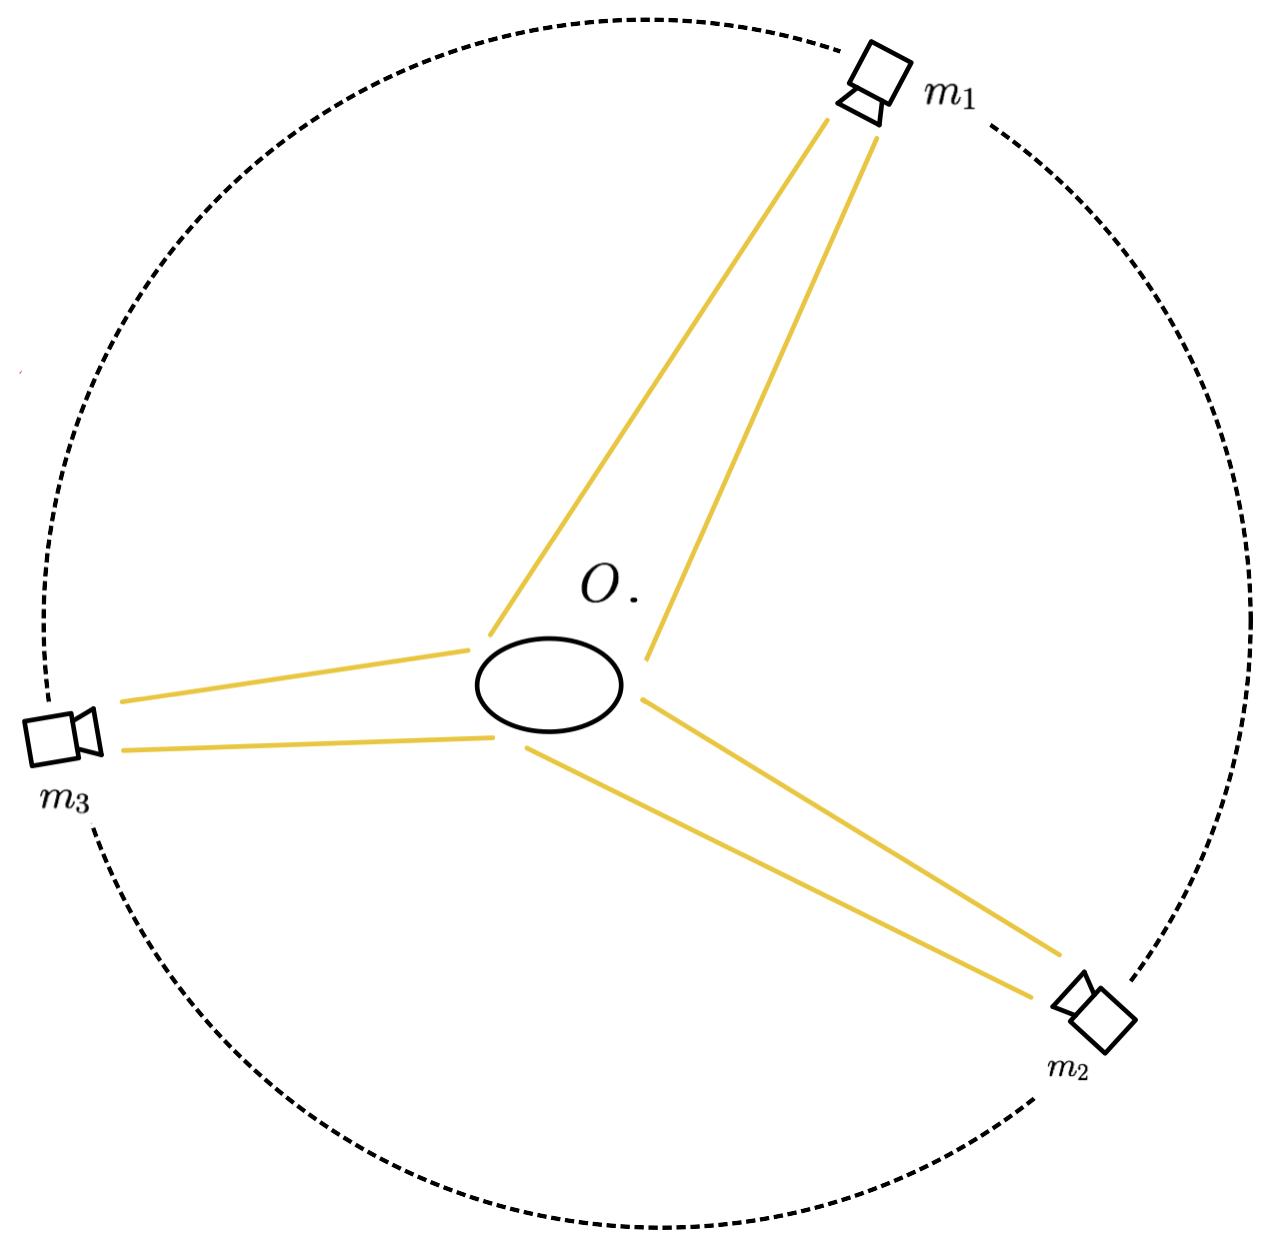
\includegraphics[scale=0.15]{问题2图示.jpg}
\caption{问题2示意图}

\label{fig:label}
\end{figure}
\section{模型假设}

\par 1.假设该平面图形足够近似椭圆,可以运用椭圆公式计算;

2.假设观测得到的长度$a$、$b$、$c$均为准确值或误差可忽略不计;

3.在第一问中,假设被测量的椭圆物体的中心在圆心,直径不超过5cm;

4.在第一问中,假设当物体足够小时,从同一摄像机所作的两条切线是平行的;

5.在第二问中,假设被测量的椭圆物体在以$O$为圆心,$20$cm 为半径的圆内。
\section{符号说明}
%本部分是对模型中使用的重要变量进行说明,一般排版时要放到一张表格中。
%注意:第一:不需要把所有变量都放到这个表里面,模型中用到的临时变量可以不放。第二:下文中首次出现这些变量时也要进行解释,不然会降低文章的可读性。
\begin{table}[h]
\centering
\begin{tabular}{C{2cm}C{12cm}C{2cm}}
\toprule[2pt]
\textbf {符号}&\textbf {定义}&\textbf {单位}\\\midrule[1pt]
$a$ & 拍摄到的第1条线段的长度  & $cm$ \\
$b$ & 拍摄到的第2条线段的长度& $cm$\\
$c$ & 拍摄到的第3条线段的长度& $cm$\\
$l$ & 椭圆的半长轴 &$cm$ \\
$k$ & 椭圆的半短轴 &$cm$ \\
$m_1$ & 第1台相机& $\backslash$\\
$m_2$ & 第2台相机& $\backslash$\\
$m_3$ & 第3台相机& $\backslash$\\
$d_1$ & 拍摄到的第一条线段与圆心的偏离程度& $cm$\\
$d_2$ & 拍摄到的第二条线段与圆心的偏离程度& $cm$\\
$d_3$ & 拍摄到的第三条线段与圆心的偏离程度& $cm$\\
$\theta$  & 相机$m_1$偏离椭圆长轴的角度 & rad\\
$S$ & 椭圆面积的近似值 & $cm^2$ \\
\bottomrule[2pt]
\end{tabular}
\label{tab:wei1}
\end{table}
注:未列出符号及重复符号以出现位置为准
\section{模型的建立与求解}
\subsection{问题模型一的建立与求解}


\subsubsection{模型的建立}
\par 以椭圆圆心$O$为坐标原点,椭圆长轴为$x$轴,短轴为$y$轴,建立平面直角坐标系。椭圆的方程为:$\frac{x^2}{l^2}+\frac{y^2}{k^2}=1$,其中 $l$ 为椭圆的半长轴长,$k$ 为椭圆的半短轴长。
\begin{figure}[h]%h可替换成t表示在页首插入图片;b页尾;p整页
\centering
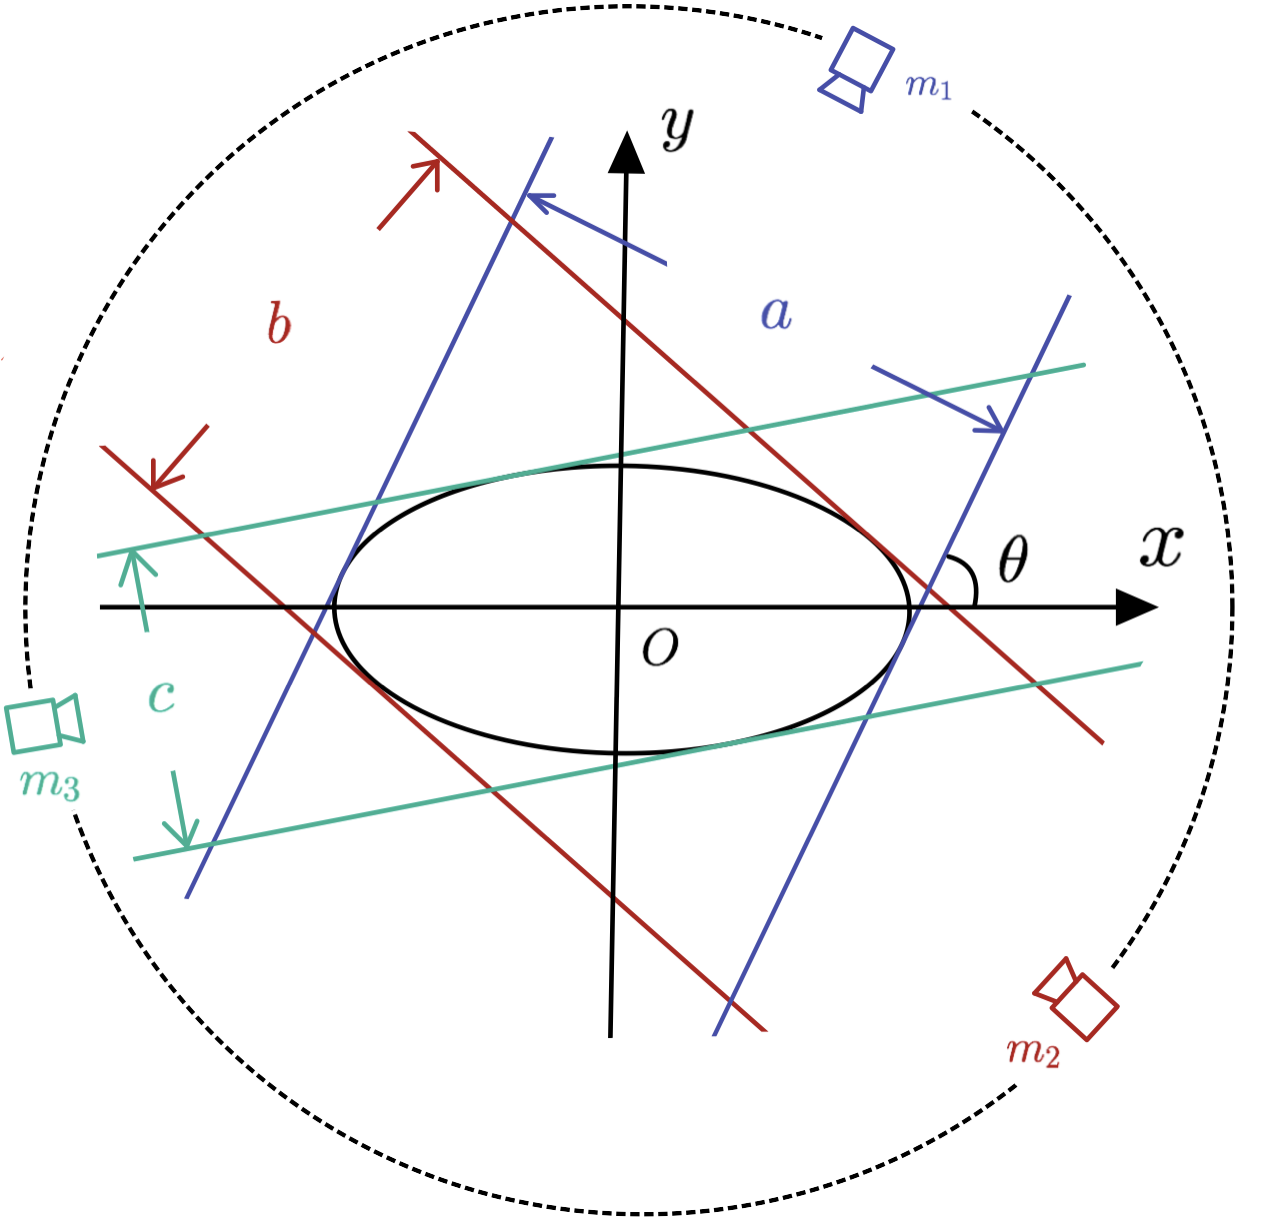
\includegraphics[scale=0.3]{模型图.png}
\caption{模型的建立}
\label{fig:label}
\end{figure}
\par 由模型假设可知,从同一台摄像机所作的两条切线是平行的,因此拍摄到的三条线段的长度$a$、$b$、$c$,即为三组平行线之间的距离。且 $m_1$ 与$x$轴偏离的角度 $\theta$ ,即为从 $m_1$ 所作的切线与$x$轴正半轴的夹角。下面建立三个已知量$(a,b,c)$与三个未知量$(l,k,\theta)$之间的方程并求解。


\subsubsection{模型的求解}
\par 由于三台摄像机被等距地放置在直径为$1$m的圆周上,故而确定一台摄像机在圆周上的位置,即可确定剩余两台摄像机的位置。假设摄像机$m_1$与圆心的连线$l_1$与$x$轴正半轴的夹角分别为$\theta(0\le \theta \le \frac{2\pi}{3} )$,则另外两台摄像机与$x$轴正半轴的夹角为$\theta -\frac{2\pi}{3}$与$\theta -\frac{4\pi}{3}$。
\begin{figure}[h]%h可替换成t表示在页首插入图片;b页尾;p整页
\centering
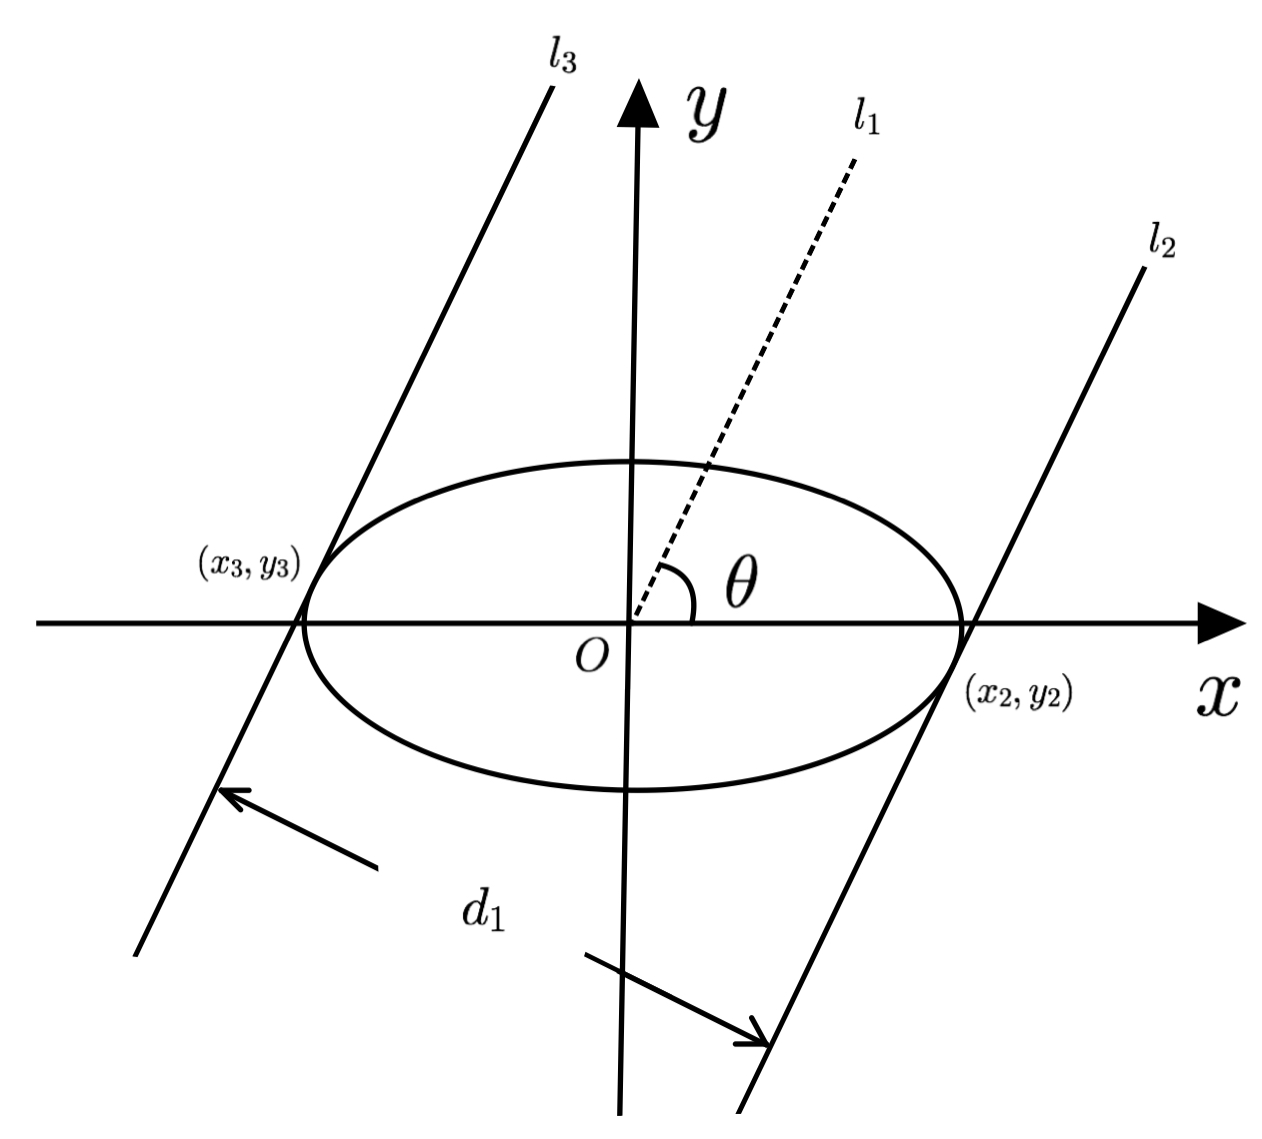
\includegraphics[scale=0.17]{问题1图示.jpg}
\caption{问题1图示}
\label{fig:label}
\end{figure}
\par 首先考虑$\theta \ne \frac{\pi}{2}$且$\theta+\frac{\pi}{3} \ne \frac{\pi}{2}$且$\theta +\frac{2\pi}{3}\ne \frac{3\pi}{2}$,则$$l_1:y=\tan\theta\cdot x$$
\par 假设所求椭圆半长轴与半短轴长分别为$l$、$k$,则对于椭圆上任意一点$(x_0,y_0)(y_0\ne0)$,过$(x_0,y_0)$且与椭圆相切的直线$l_0$的方程为$$l_0:\frac{x_0x}{l^2}+\frac{y_0y}{k^2}=1$$则$l_0$的斜率为$-\frac{x_0k^2}{y_0l^2}$。
\par 设与$l_1$平行且与椭圆相交的直线分别为$l_2$、$l_3$,它们与椭圆的切点分别为$(x_2,y_2)$、$(x_3,y_3)$,则由$l_1$与$l_2$、$l_3$的斜率相等可得:
\begin{equation}
\tan\theta=-\frac{x_2k^2}{y_2l^2}=-\frac{x_3k^2}{y_3l^2}
\end{equation}
\par 由于$(x_2,y_2)$、$(x_3,y_3)$为椭圆上两点,满足方程
\begin{equation}
\begin{align*}
\frac{x_2^2}{l^2}+\frac{y_2^2}{k^2}&=1 \\
 \frac{x_3^2}{l^2}+\frac{y_3^2}{k^2}&=1
\end{align*}
\end{equation}
\par 由$(1)(2)$两式可得:
\begin{equation}
\left\{
\begin{aligned}
x_2^2=x_3^2=\frac{l^4\tan^2\theta}{l^2\tan^2\theta+k^2} \\
y_2^2=y_3^2=\frac{k^4}{l^2\tan^2\theta+k^2}
\end{aligned}
\right.
\end{equation}
\par 由$l_2$的直线方程为$$l_2:\frac{x_2x}{l^2}+\frac{y_2y}{k^2}=1$$
得$l_2$与$l_3$直线之间的距离(即为$(x_3,y_3)$到$l_2$的距离)$d_1$满足:
\begin{align*}
d_1^2&= \frac{|\frac{x_2x_3}{l^2}+\frac{y_2y_3}{k^2}-1|^2}{\frac{x_2^2}{l^4}+\frac{y_2^2}{k^4}}\\
 &=\frac{|-\frac{x_2^2}{l^2}-\frac{y_2^2}{k^2}-1|^2}{\frac{x_2^2}{l^4}+\frac{y_2^2}{k^4}}\\
 &=\frac{4}{\frac{x_2^2}{l^4}+\frac{y_2^2}{k^4}}
\end{align*}
\par 将(3)代入可得:
$$d_1^2=\frac{4(l^2\tan^2\theta+k^2)}{1+\tan^2\theta}$$
\par 由于$d$即为摄像机所得的线段长度,故而得到三个方程:
\begin{equation}
\left\{
\begin{aligned}
a&=2\sqrt{\frac{l^2\tan^2\theta+k^2}{1+\tan^2\theta}}\\
b&=2\sqrt{\frac{l^2\tan^2(\theta+\frac{\pi}{3})+k^2}{1+\tan^2(\theta+\frac{\pi}{3})}}\\
c&=2\sqrt{\frac{l^2\tan^2(\theta+\frac{2\pi}{3})+k^2}{1+\tan^2(\theta+\frac{2\pi}{3})}}

\end{aligned}
\right.
\end{equation}
\par 再考虑$\theta=\frac{\pi}{2}$,显然有:
\begin{equation}
\left\{
\begin{aligned}
a&=2l\\
b&=\sqrt{l^2+3k^2}\\
c&=\sqrt{l^2+3k^2}
\end{aligned}
\right.
\end{equation}
\par 再考虑$\theta=\frac{\pi}{6}$,显然有:

\begin{equation}
\left\{
\begin{aligned}
a&=\sqrt{l^2+3k^2}\\
b&=2l\\
c&=\sqrt{l^2+3k^2}
\end{aligned}
\right.
\end{equation}

\par 最后考虑$\theta=\frac{5\pi}{6}$,显然有:

\begin{equation}
\left\{
\begin{aligned}
a&=\sqrt{l^2+3k^2}\\
b&=\sqrt{l^2+3k^2}\\
c&=2l
\end{aligned}
\right.
\end{equation}
\par 综上所述:当$a,b,c$互不相等时,可利用$(4)$进行求解,而$a,b,c$中存在两个值相等时,可视相等情况分别利用$(5)(6)(7)$求解。
\par 下利用MATLAB中$vpasolve$函数对方程进行求解:$vpasolve$函数可以求得代数方程式的数值解。对于含有$m$个未知数$[x_1,x_2,...,x_m]$与$n$个等式方程组$[eq_1,eq_2,...,eq_n]$,函数$vpasolve([eq_1,...,eq_n],[x_1,...,x_m],$\\$X_0)$可以返回方程的数值解,其中$X_0$为未知数的初值或者数值解所在的区间。
\par 在MATLAB中执行以下命令:
\begin{breakablealgorithm}
        \caption{通过$a,b,c$求解椭圆面积$S$的算法}
        \begin{algorithmic}[1] %每行显示行号
            \Require $a,b,c$
            \Ensure  $S$
                    \If {$(a=b\wedge b<\frac{c}{2})\vee (a=c\wedge a<\frac{b}{2})\vee(b=c\wedge b<\frac{a}{2})$}
                    \State return $ -1;$
                    \EndIf
                    \If {$a=b\wedge b=c$}
                    \State $S=\frac{a^2\pi}{4};$
                    \State return $S$
                    \EndIf
                    \If {$a=b\wedge b\ne c$}
                    \State $l=\frac{c}{2};$
                    \State $k=\sqrt{\frac{b^2-l^2}{3}};$
                    \State $S=lk\pi;$
                    \State return $S$;
                    \EndIf
                    \If {$a=c\wedge b\ne c$}
                    \State $l=\frac{b}{2};$
                    \State $k=\sqrt{\frac{a^2-l^2}{3}};$
                    \State $S=lk\pi;$
                    \State return $S$;
                    \EndIf
                    \If {$b=c\wedge a\ne c$}
                    \State $l=\frac{a}{2};$
                    \State $k=\sqrt{\frac{b^2-l^2}{3}};$
                    \State $S=lk\pi;$
                    \State return $S$;
                    \EndIf 
                    \If{$a\ne b\wedge b\ne c\wedge c\ne a$}
                    \State $solve\ equations$
                    \State $a=2\sqrt{\frac{l^2\tan^2\theta+k^2}{1+\tan^2\theta}}$
                    \State $b=2\sqrt{\frac{l^2\tan^2(\theta+\frac{\pi}{3})+k^2}{1+\tan^2(\theta+\frac{\pi}{3})}}$
                    \State $c=2\sqrt{\frac{l^2\tan^2(\theta+\frac{2\pi}{3})+k^2}{1+\tan^2(\theta+\frac{2\pi}{3})}}$           
                    \If {$l\ is\ not\ a\ real\ number$ or $k\ is\  not\  a\  real\  number$}
                    \State return$\ -1;$
                    \Else 
                    \State $S=lk\pi;$
                    \State return $S;$
                    \EndElse
                    \EndIf
                    \EndIf

     \end{algorithmic}
    \end{breakablealgorithm}

\par 通过该程序即可由输入$a$、$b$、$c$得到面积$S$的数值解,无解时返回$-1$。
\par 下面考虑在MATLAB中使用$solve$函数求得$l,k,\theta$的显式解:$solve$函数与$vpasolve$函数的用法与功能类似,$solve$函数还能模拟人工运算求得函数的公式解。
\par 在MATLAB中尝试使用$solve$函数求解方程(4),未得到显式解。
~\\
\par 再考虑所拍摄的物体为直线或圆的情况:
\begin{itemize}
  \item [1)] 所拍摄物体为线段:    
\par 保持上述公式推导不变,取$k=0$,则可得到
\begin{equation}
\left\{
\begin{aligned}
a&=2l\sin\ \theta\\
b&=2l|\sin(\theta+\frac{\pi}{3})|\\
c&=2l|\sin(\theta+\frac{2\pi}{3})|
\end{aligned}
\right.
\end{equation}
若$\theta\in[0,\frac{\pi}{3})$,此时$b$、$c$满足关系式:
\begin{equation}
\nonumber
\left\{
\begin{aligned}
b+c&=2\sqrt{3}\ l\cos\ \theta\\
b-c&=2l\sin\ \theta=a
\end{aligned}
\right.
\end{equation}
\par 利用$a$、$b$、$c$表示$l$、$\theta$得:

\begin{equation}
\nonumber
\left\{
\begin{aligned}
l^2&=\frac{(b+c)^2+3a^2}{12}\\
\sin^2\theta&=\frac{3(b-c)^2}{3a^2+(b+c)^2}
\end{aligned}
\right.
\end{equation}
\par 回代入$(8)$得$$a=b-c$$
若$\theta\in[\frac{\pi}{3},\frac{2\pi}{3}]$,此时$b$、$c$满足关系式:
\begin{equation}
\nonumber
\left\{
\begin{aligned}
b+c&=2l\sin\theta=a\\
b-c&=2\sqrt{3}\ l\cos\theta
\end{aligned}
\right.
\end{equation}
\par 利用$a$、$b$、$c$表示$l$、$\theta$得:

\begin{equation}
\nonumber
\left\{
\begin{aligned}
l^2&=\frac{(b-c)^2+3a^2}{12}\\
\sin^2\theta&=\frac{3a^2}{3a^2+(b-c)^2}
\end{aligned}
\right.
\end{equation}
\par 回代入$(8)$得$$a=b+c$$
  \item [2)] 所拍摄物体为圆:
\par 将$l=k$代入$(4)$即可得:$$a=b=c$$
\end{itemize}

\subsubsection{结果展示}
\par 模拟偏离角度分别为$\frac{\pi}{12}$,$\frac{\pi}{4}$,$\frac{3\pi}{4}$和$\frac{11\pi}{12}$的情况下,每组真实的半长轴半短轴分别取相同的六组数据,为$(0.5,1),(1,1),(0.5,2),(1,2),(0.5,3),(1,3)$(单位\ cm)。此时,观测到的三条线段长度$a,b,c$和由MATLAB程序$solve1.m$解出的面积近似数据如下表所示:

\begin{table}[h]
\centering
\caption{不同情况下近似出的椭圆面积}
\begin{tabular}{C{4cm}C{5cm}C{4.5cm}}
\toprule[2pt]
\textbf{$(l,k,\theta)$}   & \textbf{$(a,b,c)$}      &  \textbf{近似面积$S$}  \\\midrule[1pt]
$(0.5,1,\frac{\pi}{12})$   & (1.0959,1.9491,1.5811)  & 1.57079632679490 \\
$(1,1,\frac{\pi}{12})$  & (2,2,2)     & 3.14159265358979 \\
$(0.5,2,\frac{\pi}{12})$ & (1.4159,3.8724,2.9155)  & 3.14159265358980 \\
$(1,2,\frac{\pi}{12})$  & (2.1918,3.8982,3.1623)  & 6.28318530717959 \\
$(0.5,3,\frac{\pi}{12})$   & (1.8288,5.8013,4.3012) & 4.71238898038470 \\
$(1,3,\frac{\pi}{12})$     & (2.4786,5.8186,4.4721)  & 9.42477796076938 \\\cdashline{1-3}[0.8pt/2pt]
$(0.5,1,\frac{\pi}{4})$    &  (1.5811,1.9491,1.0959) &  1.57079632679490  \\
$(1,1,\frac{\pi}{4})$      &    (2,2,2)  &   3.14159265358979         \\
$(0.5,2,\frac{\pi}{4})$    &  (2.9155,3.8724,1.4159)  &  3.14159265358980   \\
$(1,2,\frac{\pi}{4})$      &     (3.1623,3.8982,2.1918)&  6.28318530717959 \\
$(0.5,3,\frac{\pi}{4})$    &   (4.3012,5.8013,1.8288)     & 4.71238898038470 \\
$(1,3,\frac{\pi}{4})$      &    (4.4721,5.8186,2.4786)     &    9.42477796076938 \\\cdashline{1-3}[0.8pt/2pt]
$(0.5,1,\frac{3\pi}{4})$   & (1.5811,1.0959,1.9491)  & 1.57079632679490  \\
$(1,1,\frac{3\pi}{4})$     & (2,2,2)& 3.14159265358979    \\
$(0.5,2,\frac{3\pi}{4})$   &  (2.9155,1.4159,3.8724) &  3.14159265358980  \\
$(1,2,\frac{3\pi}{4})$     & (3.1623,2.1918,3.8982)   &   6.28318530717959 \\
$(0.5,3,\frac{3\pi}{4})$   &(4.3012,1.8288,5.8013)  &   4.71238898038470 \\
$(1,3,\frac{3\pi}{4})$     & (4.4721,2.4786,5.8186)   &  9.42477796076938 \\\cdashline{1-3}[0.8pt/2pt]
$(0.5,1,\frac{11\pi}{12})$ &(1.0959,1.5811,1.9491) &  1.57079632679490  \\
$(1,1,\frac{11\pi}{12})$   &   (2,2,2)   & 3.14159265358979 \\
$(0.5,2,\frac{11\pi}{12})$ & (1.4159,2.9155,3.8724)& 3.14159265358980 \\
$(1,2,\frac{11\pi}{12})$   &(2.1918,3.1623,3.8982) & 6.28318530717959 \\
$(0.5,3,\frac{11\pi}{12})$ & (1.8288,4.3012,5.8013) &  4.71238898038470 \\
$(1,3,\frac{11\pi}{12})$   &  (2.4786,4.4721,5.8186)   &  9.42477796076938 \\
\bottomrule[2pt]
\end{tabular}
\label{tab:wei1}
\end{table}

\par 由上表可见,不论角度$\theta$为何值,只要真实的半长轴$l$、半短轴$k$数据确定,则观察到的三条线段的长度也固定(仅$a,b,c$顺序改变),进而得到的近似面积值$S$也是相同的。在下一部分模型检验中我们将分析:在确定$l$,$k$时,该模型得到的$S$之所以相同是因为其与真实的面积$\pi lk$误差趋近于0,而真实面积仅有$l$和$k$决定。
\subsection{问题二模型的建立与求解}

\subsubsection{模型的建立}
\par 以椭圆圆心$O$为坐标原点,椭圆长轴所在直线为$x$轴,短轴所在直线为$y$轴,建立平面直角坐标系。椭圆的方程为$$\frac{x^2}{l^2}+\frac{y^2}{k^2}=1$$其中$l$为椭圆的半长轴长,$k$为椭圆的半短轴长。
\par 由于摄像机所在大圆圆心与$O$并不重合,假设圆心$O$坐标为$(x_0,y_0)$,确定一台摄像机$m_1$与$O$的连线与$x$轴正半轴所成的角度为$\theta$,则$m_1$的坐标为$(x_0+50\cos\theta,y_0+50\sin\theta)$。
\par 由于摄像机与椭圆的距离较近,无法采用第一题切线平行假设,于是从$m_1$引椭圆的两条切线,切点分别为$T_1$、$T_2$,则线段$T_1T_2$在垂直于$Om_1$的直线上的投影即为观测所得的长度$a$,$T_1$到直线$Om_1$的距离即为观测中线段端点$T_1$到圆心的距离,而$T_2$到直线$Om_1$的距离即为观测中线段端点$T_2$到圆心的距离。在刻画观测中所得的线段端点的偏离程度时,若观测中所得到的圆心在线段上,则采用摄像机所拍摄到的圆心到两端点的距离之差的绝对值作为偏离程度;若观测所得到的圆心在线段外,则采用摄像机所拍摄到的圆心到两端点的距离之和作为偏离程度。从另一个角度来说,在观测中分别测量两个端点到圆心的距离后,两端距离之和与之差的绝对值就是所要求的观测线段长度与偏离长度,具体的对应方式视线段与圆心的相对关系决定。
\begin{figure}[h]%h可替换成t表示在页首插入图片;b页尾;p整页
\centering
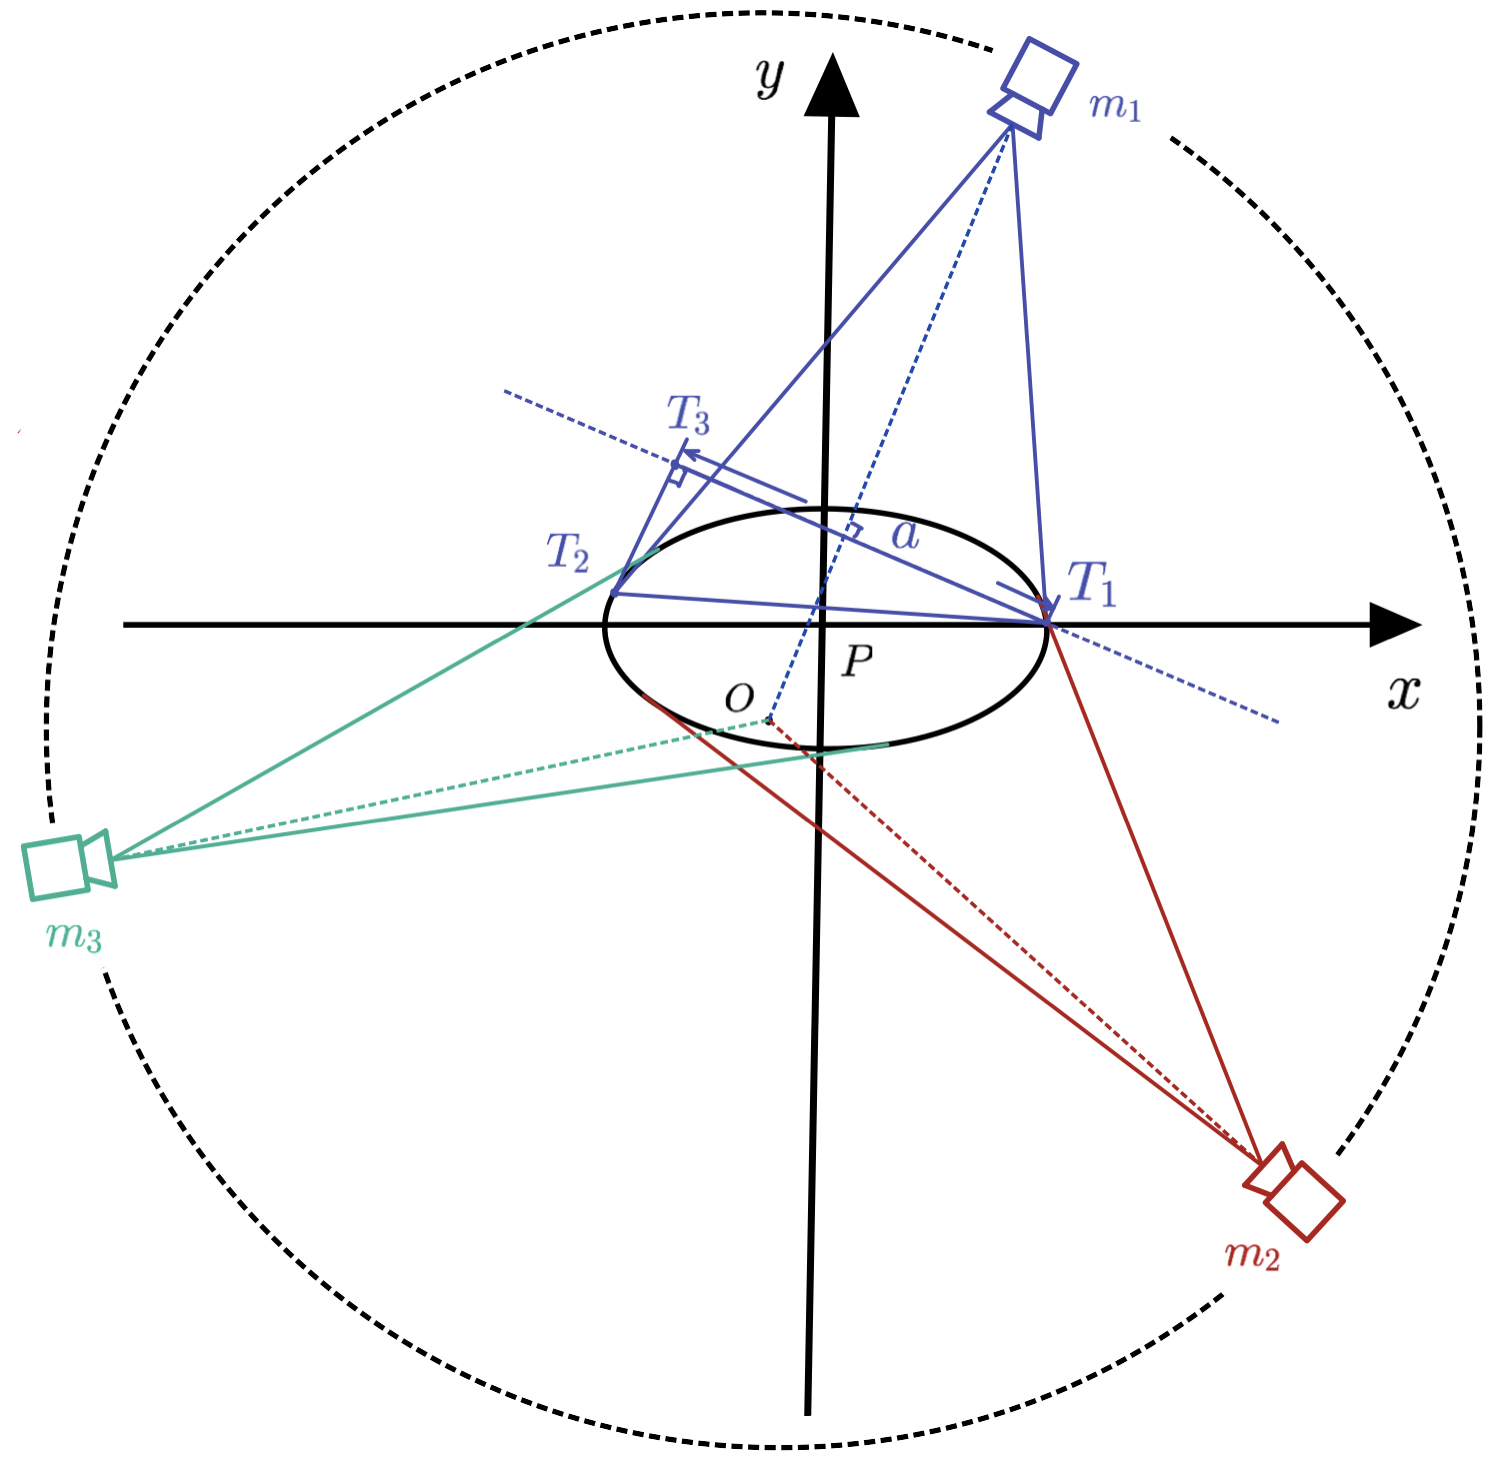
\includegraphics[scale=0.17]{问题2建模.jpg}
\caption{问题2模型的建立}
\label{fig:label}
\end{figure}

\subsubsection{模型的求解}
记大圆的圆心坐标为$(x_0,y_0)$,第一台摄像机$m_1$与圆心连线与$x$轴夹角为$\theta$,则$m_1$坐标为$(x_0+50\cos\theta,y_0+50\sin\theta)$,设为$(x_1,y_1)$,则过$m_1$所作的椭圆的两条切线与椭圆的切点的连线方程为:$$\frac{x_1x}{l^2}+\frac{y_1y}{k^2}=1$$
\par 联立方程组
\begin{equation}
\nonumber
\left\{
\begin{aligned}
\frac{x_1x}{l^2}+\frac{y_1y}{k^2}=1 \\
\frac{x^2}{l^2}+\frac{y^2}{k^2}=1
\end{aligned}
\right.
\end{equation}
\par 利用MATLAB中$solve$函数求解得到由$m_1$作切线得到的用$l,k,x_0,y_0$表达两个切点$T_1(x_2,y_2)$、$T_2(x_3,y_3)$坐标的表达式。
\par 由问题一的模型求解中对$solve$函数的介绍可得,$solve$函数可以解得满足方程的所有未知量的表达式。通过下述算法可以利用MATLAB解得两个点的表达式,存入$solx_{11},soly_{11},solx_{12},soly_{12}$中:
\begin{breakablealgorithm}
        \caption{通过联立方程求解切点坐标}
        \begin{algorithmic}[1] %每行显示行号
            \Require $x_0,y_0,l,k$
            \Ensure  $x_2,x_3,y_2,y_3$
                    \State  $solve\ equations$
                    \State $eqn_1=\frac{(x_0+50\cos\theta)x_2}{l^2}+\frac{(y_0+50\sin\theta)y_2}{k^2}==1$
                    \State $eqn_2=\frac{x_{2}^2}{l^2}+\frac{y_{2}^2}{k^2}==1$
                    \State $eqnn_1=\frac{(x_0+50\cos\theta)x_3}{l^2}+\frac{(y_0+50\sin\theta)y_3}{k^2}==1$
                    \State $eqnn_2=\frac{x_3^2}{l^2}+\frac{y^3}{k^2}==1$
                    \State $[solx_{11},soly_{11},solx_{12},soly_{12}]= solve([eqn_1,eqn_2,eqnn_1,eqnn_2],[x_2,y_2,x_3,y_3])$
                    \For {$i_1=1:4$}
                    \If {$(solx_{11}(i_1)\ne solx_{12}(i_1))\wedge(soly_{11}(i_1)\ne soly_{12}(i_1))$}
                    \State $solx_{11}=solx_{11}(i_1);$
                    \State $soly_{11}=soly_{11}(i_1);$
                    \State $solx_{12}=solx_{12}(i_1);$
                    \State $soly_{12}=soly_{12}(i_1);$
                    \State break;
                    \EndIf
                    \EndFor
     \end{algorithmic}
    \end{breakablealgorithm}
\par 由弦长公式,得到割线$T_1T_2$的长度$L$:
\begin{equation}
\begin{aligned}
L^2=(1+\frac{k^4x_{1}^2}{l^4y_{1}^2})(x_2-x_3)^2
\end{aligned}
\end{equation}
\par 进一步,利用直角三角形$T_1T_2T_3$的各边关系,得到$T_1T_3$即摄像机拍到的线段$a$的表达式为:
\begin{equation}
\begin{aligned}
a&=L·|\cos(\phi-\theta-\frac{\pi}{2})|\\
&=L·|\sin(\phi-\theta)|
\end{aligned}
\end{equation}
\par 其中,$\phi=\arctan(-\frac{k^2x_1}{l^2y_1})$,为割线$T_1T_2$与$x$轴正方向的夹角。
\par 同样的,可以考虑$m_2$与$m_3$观测到的线段长度,将上式中$\theta$分别替换为$\theta+\frac{2\pi}{3}$以及$\theta+\frac{4\pi}{3}$可以得到$b$、$c$。由此可用$l,k,x_0,y_0,\theta$得到$a,b,c$的表达式,由观测所得的$a$、$b$、$c$得到三个方程。
\begin{figure}[h]%h可替换成t表示在页首插入图片;b页尾;p整页
\centering
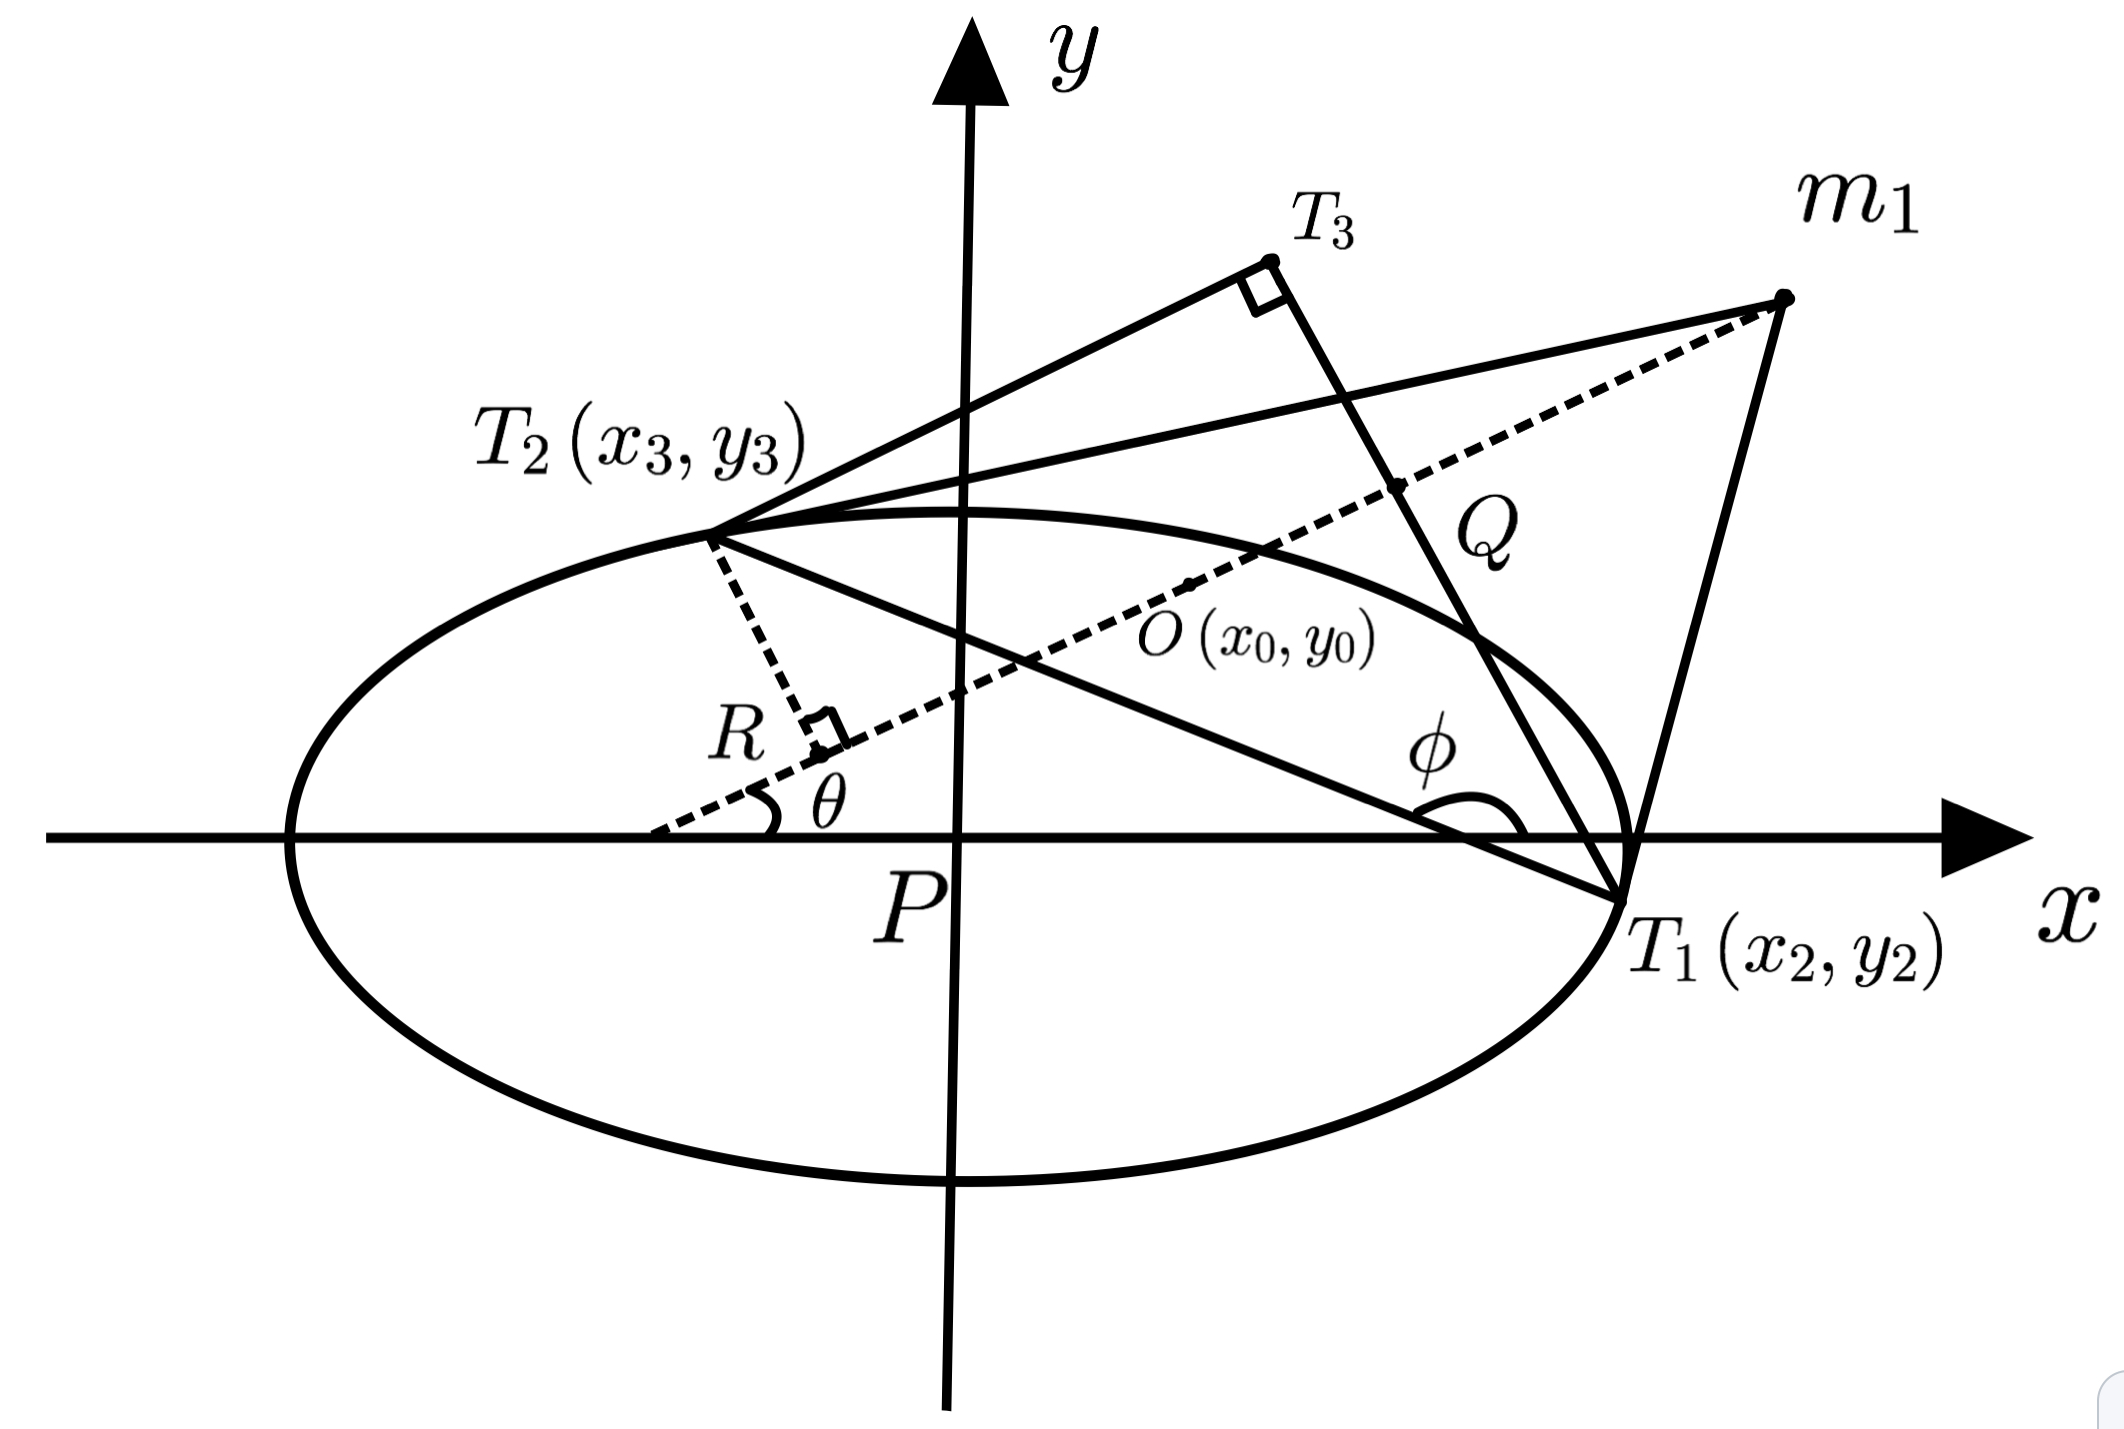
\includegraphics[scale=0.17]{问题2.jpg}
\caption{问题2图示}
\label{fig:label}
\end{figure}
\par 下面考虑照片上所反映的线段的端点偏离圆心$O$的程度。作$Om_1$的延长线与$T_1T_3$交于点Q,则$QT_1$为照片上所反映的线段的端点$T_1$到圆心$O$的距离。下面考虑$QT_1$的长度:
\par $OQ$的直线方程为:$$y-y_0=\tan\theta(x-x_0)$$
\par $T_1Q$的直线方程为:$$\cos\theta(x-x_2)+\sin\theta(y-y_2)=0$$
\par 故而两条直线的交点$Q(x_4,y_4)$坐标为
\begin{equation}
\begin{aligned}
x_4&=\frac{\cos\theta x_2-\sin\theta y_0+\sin\theta \tan\theta x_0+\sin\theta y_2}{\cos\theta+\sin\theta \tan\theta}\\
y_4&=\frac{\sin\theta x_2-\sin\theta x_0+\cos\theta y_0+\sin\theta \tan\theta y_2}{\cos\theta+\sin\theta \tan\theta}
\end{aligned}
\end{equation}
\par 故而
$$T_1Q=\sqrt{(x_4-x_2)^2+(y_4-y_2)^2}$$
\par 同理可以得到另一个端点$T_2$偏离圆心的距离$T_2R=\sqrt{(x_5-x_3)^2+(y_5-y_3)^2}$,其中$R$的垂点$(x_5,y_5)$为:
\begin{equation}
\begin{aligned}
x_4&=\frac{\cos\theta x_3-\sin\theta y_0+\sin\theta \tan\theta x_0+\sin\theta y_3}{\cos\theta+\sin\theta \tan\theta}\\
y_4&=\frac{\sin\theta x_3-\sin\theta x_0+\cos\theta y_0+\sin\theta \tan\theta y_3}{\cos\theta+\sin\theta \tan\theta}
\end{aligned}
\end{equation}
\par 在刻画线段端点偏离圆心的程度时,考虑两种情况:
\par 若圆心在线段外,则采用摄像机中所拍摄的两个线段端点到圆心的距离之和,即$$d_1=T_1Q+T_2R$$
\par 若圆心在线段上,则采用摄像机中所拍摄的两个线段端点到圆心距离之差的绝对值,即$$d_1=|T_1Q-T_2R|$$
\par 同时考虑另外两个摄像机中所观测到的偏离程度,将上式中$\theta$分别替换为$\theta+\frac{2\pi}{3}$以及$\theta+\frac{4\pi}{3}$可以得到$d_2$、$d_3$的表达式。根据所观测到的线段与圆心的位置关系带入相应的关系式,用$l,k,x_0,y_0,\theta$表示$d_1$、$d_2$、$d_3$,代入$d_1$、$d_2$、$d_3$的观测值,得到三个方程。
\par 联立六个方程:
\begin{equation}
\nonumber
\left\{
\begin{aligned}
a&=\sqrt{1+\frac{k^4x_1^2}{l^4y_1^2}}|(x_2-x_3)\sin(\phi-\theta)|\\
b&=\sqrt{1+\frac{k^4m_1^2}{l^4n_1^2}}|(m_2-m_3)\sin(\alpha -\theta-\frac{2\pi}{3})|\\
c&=\sqrt{1+\frac{k^4p_1^2}{l^4q_1^2}}|(p_6-q_7)\sin(\beta -\theta)-\frac{4\pi}{3})|\\
d_1^{+}&=\sqrt{(x_4-x_2)^2+(y_4-y_2)^2}+\sqrt{(x_5-x_3)^2+(y_5-y_3)^2}\\
d_2^{+}&=\sqrt{(m_4-m_2)^2+(n_4-n_2)^2}+\sqrt{(m_5-m_3)^2+(n_5-n_3)^2}\\
d_3^{+}&=\sqrt{(p_4-p_2)^2+(q_4-q_2)^2}+\sqrt{(p_5-p_3)^2+(q_5-q_3)^2}\\
d_1^{-}&=|\sqrt{(x_4-x_2)^2+(y_4-y_2)^2}-\sqrt{(x_5-x_3)^2+(y_5-y_3)^2}|\\
d_2^{-}&=|\sqrt{(m_4-m_2)^2+(n_4-n_2)^2}-\sqrt{(m_5-m_3)^2+(n_5-n_3)^2}|\\
d_3^{-}&=|\sqrt{(p_4-p_2)^2+(q_4-q_2)^2}-\sqrt{(p_5-p_3)^2+(q_5-q_3)^2}|\\
\end{aligned}
\right.
\end{equation}
\par {\bf 注:}在后六个式子中只需根据线段与圆心的关系选择三个公式进行计算;$(m_i,n_i),(p_i,q_i),\alpha ,\beta$与$(x_i,y_i),\phi$含义类似,为其它两个摄像头所产生的切点等。
\par 由于三台摄像机可以提供六个等式,代入$(a,b,c,d_1,d_2,d_3)$的值以及各中间变量的表达式,利用MATLAB中的$vpasolve$函数可求得方程的解。
~\\
\par 

\section{模型的分析与检验}
\subsection{问题一模型的分析与检验}
\par 我们通过改变椭圆实际的长短轴长度$l$,$k$以及第一台摄像机关于长轴的角度$\theta$来观察问题一中由$a,b,c$构造出来的椭圆近似面积与由椭圆面积公式计算出的面积之差。当偏离角度$\theta$分别为$\frac{\pi}{12}$,$\frac{\pi}{4}$,$\frac{3\pi}{4}$,$\frac{11\pi}{12}$时,我们运用MATLAB中的$mesh$函数绘制关于$l$和$k$双变量,以面积误差为因变量的三维图,具体的误差变化如下图所示。
\begin{figure}[h]
\centering
\begin{minipage}[t]{0.48\textwidth}
\centering
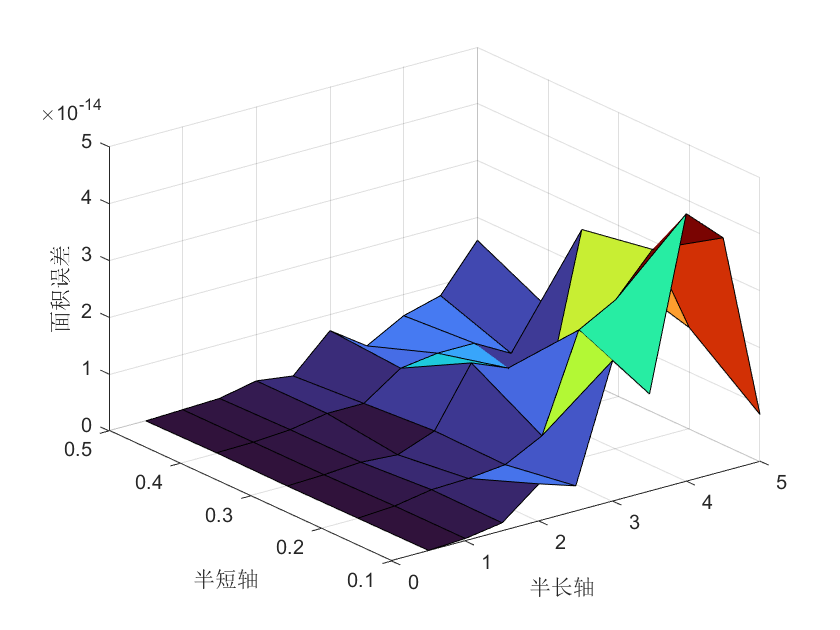
\includegraphics[width=9cm]{误差3.png}
\caption{$\theta=\frac{\pi}{12}$}
\end{minipage}
\begin{minipage}[t]{0.48\textwidth}
\centering
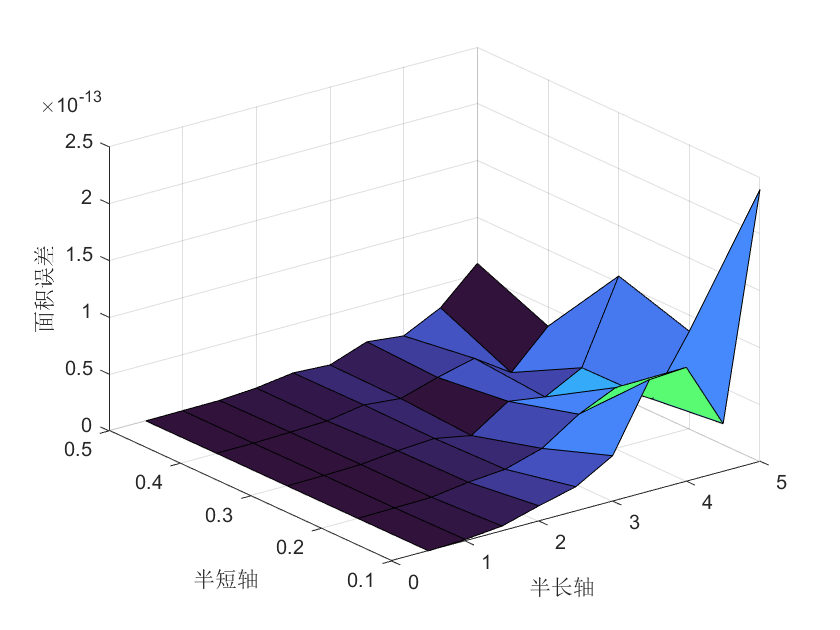
\includegraphics[width=9cm]{误差1.png}
\caption{$\theta=\frac{\pi}{4}$}
\end{minipage}
\end{figure}
\begin{figure}[h]
\centering
\begin{minipage}[t]{0.48\textwidth}
\centering
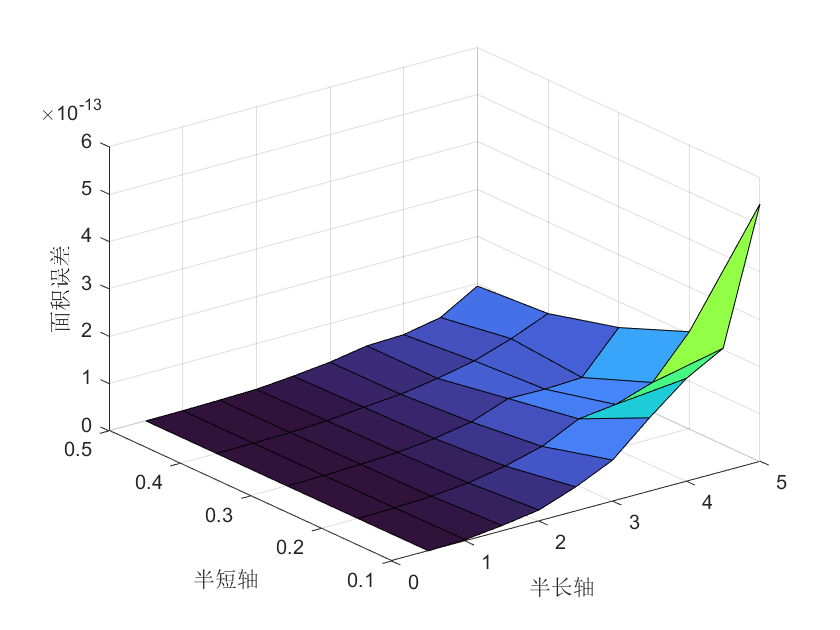
\includegraphics[width=9cm]{误差2.png}
\caption{$\theta=\frac{3\pi}{4}$}
\end{minipage}
\begin{minipage}[t]{0.48\textwidth}
\centering
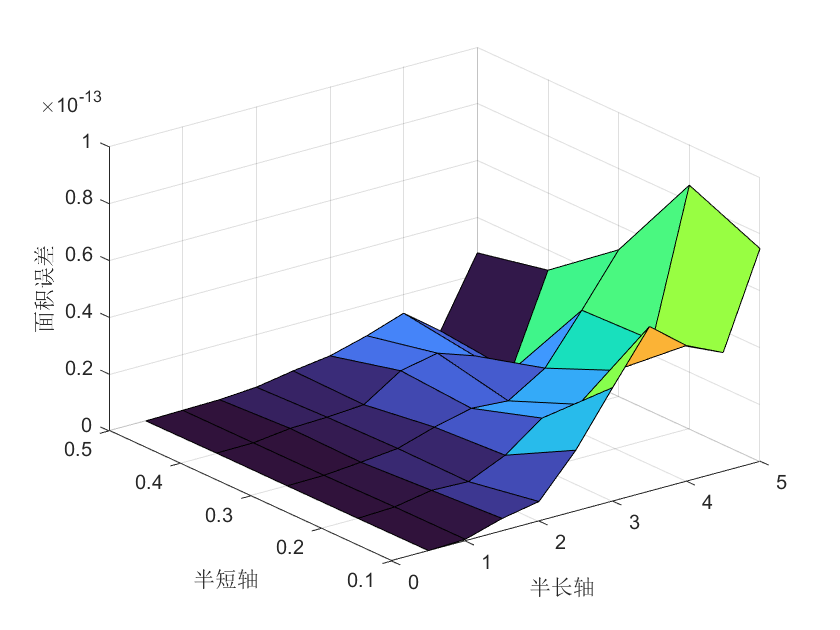
\includegraphics[width=9cm]{误差4.png}
\caption{$\theta=\frac{11\pi}{12}$}
\end{minipage}
\end{figure}
\par 观察上面四张图,在四种偏离情况下,随着$l$,$k$变化,面积误差数量级均控制在$10^{-13}$以内,相对误差不超过$10^{-11}\%$。这代表$l$,$k$和$\theta$对结果的影响不大,说明了我们模型的准确性。
\subsection{问题二模型的分析与检验}
\par 考虑到问题二模型的求解效率不高,我们在误差检验时先任意选定一组初始值 $(l,k,\theta,x_0,y_0)$ 进行求解后,依次对于 $\theta$,$(x_0,y_0)$ 以及 $(l,k)$ 这几组变量进行适当调整,再进行求解。每次求解后,记录输入参数 $(a,b,c,d_1,d_2,d_3)$ 并计算误差。误差检验结果如下表所示。
\begin{table}[h]
\centering
\caption{不同情况下近似出的椭圆面积}
\begin{tabular}{C{5cm}C{5cm}C{3cm}}
\toprule[2pt]
\textbf{$(a,b,c)$}   & \textbf{$(d_1,d_2,d_3)$}      &  \textbf{近似面积$S$}  \\\midrule[1pt]
$(3.9058,3.9058,3.979)$   & (17.2878,17.2878,0)  & 12.5663823674 \\
$(3.9479,3.9645,3.9009)$  & (9.9771,9.9886,19.9695)     & 12.5664235672 \\
$(3.9065,3.979,3.9052)$ & (17.1622,0.2486,17.4109)  & 12.5663726381 \\
$(3.9302,3.9302,3.9763)$  & (17.2984,17.2984,0)  & 12.5664038279 \\\cdashline{1-3}[0.8pt/2pt]

$(3.9716,3.9812,3.9960)$   & (10.9100,7.9846,2.9249) & 12.5663948268 \\
$(3.9935,3.9858,3.9736)$     & (2.9210,7.9884,10.9109)  & 12.5664027381 \\
$(3.9948,3.9739,3.9613)$    &  (2.9210,7.9894,10.9036) &  12.5673827928 \\
$(3.9747,3.9863,3.9938)$      &    (10.9117,7.9894,2.9218)  &   12.5663923817         \\\cdashline{1-3}[0.8pt/2pt]

$(1.5297,1.0356,1.3422)$    &  (1.9815,1.9461,3.9644)  &  1.0773418573   \\
$(1.0590,0.9316,1.2891)$      &     (1.4606,1.3392,2.9014)&  1.0773420347 \\
$(1.0535,0.8876,1.2696)$    &   (1.4554,1.2953,2.9014)     & 1.0773428371 \\
$(2.4838,2.0336,2.7795)$      &    (1.9560,0.7295,2.7775)     &   5.2686110483\\

\bottomrule[2pt]
\end{tabular}
\label{tab:wei1}
\end{table}
\par 由于我们得到测试数据的方法是确定参数 $(l,k,\theta,x_0,y_0)$ 后进行作图,然后测量出 $(a,b,c,d_1,d_2,d_3)$,因此在原始数据上会存在一定的舍入误差。尽管如此,在所有的测试数据中,估计出的椭圆面积与设定数值的误差都控制在了题目要求的范围之内。





\section{模型的评价与改进}
\subsection{模型的优点}
\par 1.问题一模型简洁、求解速度快、求解精度高。在误差检验中已经指出,问题一的模型可以将绝对误差控制在 $10^{-13}$ 以内,相对误差控制在 $10^{-11}$ 以内。同时,问题一的模型求解一组 $(a,b,c)$ 的平均时间可以控制在 $0.2$s 以内。

2.问题一的模型考虑了椭圆退化为圆、退化为直线以及 $\tan\ \theta$ 不存在的特殊情况,不会出现方程无解的情形。问题一模型的求解方式为MATLAB编程求解,因此对于上述特殊情况,在程序中都一一做了判断,再进行求解。
问题二的模型贴近实际情况。由于椭圆在以$ O $为圆心,$20$cm为半径的圆里,因此舍弃了问题一中对同一摄像机所作切线平行的假设,认为同一摄像机所作的两条切线是从摄像机上的同一点发出的。

3.模型除了计算椭圆面积,还可以求出所有的未知参数:在问题一的模型中,不仅可以计算出椭圆的面积,还可以计算出三台摄像机与椭圆长轴的偏离角度;在问题二的模型中,可以计算出摄像机与椭圆长轴的偏离角度以及椭圆圆心与$ O $的偏离程度。



\subsection{模型的缺点}
\par 1. 问题一模型关于同一摄像机所作的切线平行的假设在大幅提高求解效率的同时,会给计算结果带来一定误差。

2. 问题二模型在舍弃了诸多假设,力求贴近实际情况的同时带来方程复杂、未知量多、求解效率低等问题。
\subsection{模型的改进}
\par 1. 在时间允许的情况下,可以省略问题一中“所作切线平行”的条件,对问题一重新进行建模。这样虽然不能求出显式解,但是在一定程度上会提高原有的计算精度。

2. 因为程序整体性强、难以拆分,导致问题二的程序运行效率低、求解时间长。故而可以考虑优化程序,提高算法效率。

3. 问题二中我们关于五个未知量建立了六个方程,说明提示条件并未充分利用。故而可以利用现有条件,进一步改进算法。
\clearpage


\begin{center}
\Large{\bf {附\qquad 录}}

\end{center}
{\bf 附录1}
\begin{lstlisting}
%问题1代码:
%solve1.m
function S = solve1(a,b,c)
if a == b && b == c %圆
    S = pi*a^2/4;
    return;
end
if a == b 
    l = c/2;
    k = sqrt((b^2-l^2)/3);
    S = pi*l*k;
    return
end
if c == b 
    l = a/2;
    k = sqrt((b^2-l^2)/3);
    S = pi*l*k;
    return
end
if a == c
    l = b/2;
    k = sqrt((a^2-l^2)/3);
    S = pi*l*k;
    return
end
syms x y z
eqn1 = 2*sqrt((x^2*(tan(z))^2+y^2)/(1+(tan(z))^2)) == a;
eqn2 = 2*sqrt((x^2*(tan(z+pi/3))^2+y^2)/(1+(tan(z+pi/3))^2)) == b;
eqn3 = 2*sqrt((x^2*(tan(z+pi*2/3))^2+y^2)/(1+(tan(z+pi*2/3))^2)) == c;
[ll,kk,theta] = vpasolve([eqn1,eqn2,eqn3],[x,y,z]);
S = abs(pi*ll*kk);
end
\end{lstlisting}
{\bf 附录2}

\begin{lstlisting}
%问题二代码:
%solve2.m
clear;clc
a = input('请输入拍摄到的第一条线段长度:\n');
b = input('请输入拍摄到的第二条线段长度:\n');
c = input('请输入拍摄到的第三条线段长度:\n');
d1 = input('请输入O与第一条线段的偏离程度(O在线段外为+,O在线段内为-):\n');
d2 = input('请输入O与第二条线段的偏离程度(O在线段外为+,O在线段内为-):\n');
d3 = input('请输入O与第三条线段的偏离程度(O在线段外为+,O在线段内为-):\n');
% 定义所有需要用到的变量
syms x11 y11 x12 y12 x21 y21 x22 y22 x31 y31 x32 y32 L K Theta x0 y0 
%xij是切点
syms phi1 phi2 phi3 d11 d12 d21 d22 d31 d32
syms xx11 yy11 xx12 yy12 xx21 yy21 xx22 yy22 xx31 yy31 xx32 yy32 
%xxij是垂足
% 求解第一台摄像机的两个切点,储存在sol_x11 sol_y11 sol_x12 sol_y12
eqn11 = x11^2/L^2 + y11^2/K^2 == 1;
eqn12 = x12^2/L^2 + y12^2/K^2 == 1;
eqnn11 = (x0+50*cos(Theta))*x11/L^2 + (y0+50*sin(Theta))*y11/K^2 == 1;
eqnn12 = (x0+50*cos(Theta))*x12/L^2 + (y0+50*sin(Theta))*y12/K^2 == 1;
[sol_x11,sol_y11,sol_x12,sol_y12] = solve([eqn11,eqn12,eqnn11,eqnn12],[x11,y11,x12,y12]);
for i1 = 1:4
    if sol_x11(i1) ~= sol_x12(i1) && sol_y11(i1) ~= sol_y12(i1)
        sol_x11 = sol_x11(i1);
        sol_y11 = sol_y11(i1);
        sol_x12 = sol_x12(i1);
        sol_y12 = sol_y12(i1);
        break;
    end
end
% 求解第二台摄像机的两个切点,储存在sol\_x21 sol\_y21 sol\_x22 sol\_y22
eqn21 = x21^2/L^2 + y21^2/K^2 == 1;
eqn22 = x22^2/L^2 + y22^2/K^2 == 1;
eqnn21 = (x0+50*cos(Theta+pi*2/3))*x21/L^2 + (y0+50*sin(Theta+pi*2/3))*y21/K^2 == 1;
eqnn22 = (x0+50*cos(Theta+pi*2/3))*x22/L^2 + (y0+50*sin(Theta+pi*2/3))*y22/K^2 == 1;
[sol_x21,sol_y21,sol_x22,sol_y22] = solve([eqn21,eqn22,eqnn21,eqnn22],[x21,y21,x22,y22]);
for i2 = 1:4
    if sol_x21(i2) ~= sol_x22(i2) && sol_y21(i2) ~= sol_y22(i2)
        sol_x21 = sol_x21(i2);
        sol_y21 = sol_y21(i2);
        sol_x22 = sol_x22(i2);
        sol_y22 = sol_y22(i2);
        break;
    end
end
% 求解第三台摄像机的两个切点,储存在sol\_x31 sol\_y31 sol\_x32 sol\_y32
eqn31 = x31^2/L^2 + y31^2/K^2 == 1;
eqn32 = x32^2/L^2 + y32^2/K^2 == 1;
eqnn31 = (x0+50*cos(Theta+pi*4/3))*x31/L^2 + (y0+50*sin(Theta+pi*4/3))*y31/K^2 == 1;
eqnn32 = (x0+50*cos(Theta+pi*4/3))*x32/L^2 + (y0+50*sin(Theta+pi*4/3))*y32/K^2 == 1;
[sol_x31,sol_y31,sol_x32,sol_y32] = solve([eqn31,eqn32,eqnn31,eqnn32],[x31,y31,x32,y32]);
for i3 = 1:4
    if sol_x31(i3) ~= sol_x32(i3) && sol_y31(i3) ~= sol_y32(i3)
        sol_x31 = sol_x31(i3);
        sol_y31 = sol_y31(i3);
        sol_x32 = sol_x32(i3);
        sol_y32 = sol_y32(i3);
        break;
    end
end
% 建立a的方程
phi1 = atan(-K^2*(x0+50*cos(Theta))/(L^2*(y0+50*sin(Theta))));
fin_eqn1 = abs(sin(phi1-Theta))*sqrt(1+K^4*(x0+50*cos(Theta))^2/(L^4*(y0+50*sin(Theta))^2))*abs(sol_x11-sol_x12) == a;
% 建立b的方程
phi2 = atan(-K^2*(x0+50*cos(Theta+pi*2/3))/(L^2*(y0+50*sin(Theta+pi*2/3))));
fin_eqn2 = abs(sin(phi2-(Theta+pi*2/3)))*sqrt(1+K^4*(x0+50*cos((Theta+pi*2/3)))^2/(L^4*(y0+50*sin((Theta+pi*2/3)))^2))*abs(sol_x21-sol_x22) == b;
% 建立c的方程
phi3 = atan(-K^2*(x0+50*cos(Theta+pi*4/3))/(L^2*(y0+50*sin(Theta+pi*4/3))));
fin_eqn3 = abs(sin(phi3-(Theta+pi*4/3)))*sqrt(1+K^4*(x0+50*cos((Theta+pi*4/3)))^2/(L^4*(y0+50*sin((Theta+pi*4/3)))^2))*abs(sol_x31-sol_x32) == c;
% 建立d1的方程
cross11_eqn1 = yy11-y0 == tan(Theta)*(xx11-x0);
cross11_eqn2 = cos(Theta)*(xx11-sol_x11) + sin(Theta)*(yy11-sol_y11) == 0;
[sol_xx11,sol_yy11] = solve([cross11_eqn1,cross11_eqn2],[xx11,yy11]);%垂足
cross12_eqn1 = yy12-y0 == tan(Theta)*(xx12-x0);
cross12_eqn2 = cos(Theta)*(xx12-sol_x12) + sin(Theta)*(yy12-sol_y12) == 0;
[sol_xx12,sol_yy12] = solve([cross12_eqn1,cross12_eqn2],[xx12,yy12]);%垂足
d11 = sqrt((sol_xx11-sol_x11)^2+(sol_yy11-sol_y11)^2);
d12 = sqrt((sol_xx12-sol_x12)^2+(sol_yy12-sol_y12)^2);
if d1 > 0
    fin_eqn11 = abs(d11+d12) == d1;
else
    fin_eqn11 = abs(d11-d12) == d1;
end
% 建立d2的方程
cross21_eqn1 = yy21-y0 == tan(Theta+pi*2/3)*(xx21-x0);
cross21_eqn2 = cos(Theta+pi*2/3)*(xx21-sol_x21) + sin(Theta+pi*2/3)*(yy21-sol_y21) == 0;
[sol_xx21,sol_yy21] = solve([cross21_eqn1,cross21_eqn2],[xx21,yy21]);%垂足
cross22_eqn1 = yy22-y0 == tan(Theta+pi*2/3)*(xx22-x0);
cross22_eqn2 = cos(Theta+pi*2/3)*(xx22-sol_x22) + sin(Theta+pi*2/3)*(yy22-sol_y22) == 0;
[sol_xx22,sol_yy22] = solve([cross22_eqn1,cross22_eqn2],[xx22,yy22]);%垂足
d21 = sqrt((sol_xx21-sol_x21)^2+(sol_yy21-sol_y21)^2);
d22 = sqrt((sol_xx22-sol_x22)^2+(sol_yy22-sol_y22)^2);
if d2 > 0
    fin_eqn22 = abs(d21+d22) == d2;
else
    fin_eqn22 = abs(d21-d22) == d2; 
end
% 建立d3的方程
cross31_eqn1 = yy31-y0 == tan(Theta+pi*4/3)*(xx31-x0);
cross31_eqn2 = cos(Theta+pi*4/3)*(xx31-sol_x31) + sin(Theta+pi*4/3)*(yy31-sol_y31) == 0;
[sol_xx31,sol_yy31] = solve([cross31_eqn1,cross31_eqn2],[xx31,yy31]);%垂足
cross32_eqn1 = yy32-y0 == tan(Theta+pi*4/3)*(xx32-x0);
cross32_eqn2 = cos(Theta+pi*4/3)*(xx32-sol_x32) + sin(Theta+pi*4/3)*(yy32-sol_y32) == 0;
[sol_xx32,sol_yy32] = solve([cross32_eqn1,cross32_eqn2],[xx32,yy32]);%垂足
d31 = sqrt((sol_xx31-sol_x31)^2+(sol_yy31-sol_y31)^2);
d32 = sqrt((sol_xx32-sol_x32)^2+(sol_yy32-sol_y32)^2);
if d3>0
    fin_eqn33 = abs(d31+d32) == d3;
else
    fin_eqn33 = abs(d31-d32) == d3;
end
% 最终求解
Range = [-20 20;-20 20;0 2*pi;0 5;0 5];
[sol_x0,sol_y0,sol_Theta,sol_L,sol_K] = vpasolve([fin_eqn1,fin_eqn2,fin_eqn3,fin_eqn11,fin_eqn22],[x0,y0,Theta,L,K],Range);
sol_L = abs(double(sol_L));
sol_K = abs(double(sol_K));
S = abs(sol_L.*sol_K)*pi;
\end{lstlisting}

\end{document}